\section{評価}
本章では、提案システムの性能評価について述べる。本評価ではボランティアコンピューティングを活用したクラウドゲーミングシステムの実現可能性を評価することを目的とする。また、提案システムが実現可能であるときそれが有用な条件は、プレイヤーPCからデータセンターよりもボランティアの提供する遊休コンピュータに接続する方がネットワーク遅延が小さい状況である。提案システムの実現可能性を評価するため、通信性能の評価および、ゲームプレイにおけるQoEを測定するためにフレームレートの評価も行う。

まず、評価を行う環境について述べる。次に、クラウドゲームサーバ/クライアント間の通信性能の評価について述べる。その後、ゲームプレイ時のフレームレートの評価について述べる。最後に評価についての考察を述べる。

\subsection{評価環境}
既存のクラウドゲーミングシステムはクラウドのデータセンター上でクラウドゲームサーバが動作している。これに対し、提案システムはボランティアが提供する遊休コンピュータ上でクラウドゲームサーバを動作させることで、プレイヤーからデータセンターまでの遅延を削減することを目指した。一般にユーザコンピュータからデータセンターへの遅延は大きくても50ms程度であるが、提案システムでのゲームプレイ中に発生する遅延がこの基準を下回るかどうかを評価する。また、提案システムの通信を実現するために組み込んだトンネリングのオーバヘッドについても評価を行う。

評価を行う環境を図\ref{fig:expenv}のように構築した。ボランティアクラウドゲーミングコントローラは用意せず、クラウドサーバ上にはEdgeVPNのリンクを確立するために必要なXMPPサーバのみを用意した。プレイヤーPCの役割を果たすsiciliaではgRPCクライアントとGamingAnywhereクライアントが動作する。また、遊休コンピュータの役割を果たすfirenzeではgRPCサーバ、GamingAnywhereサーバおよびゲームが動作する。siciliaとfirenzeはそれぞれUbuntu20.04で動作するマシンを用い、1Gbpsのリンクを持つネットワークで接続した。このリンクに遅延挿入や帯域制限をかけることで様々なネットワーク環境での評価を実現する。

\begin{figure*}[t]
    \centering
    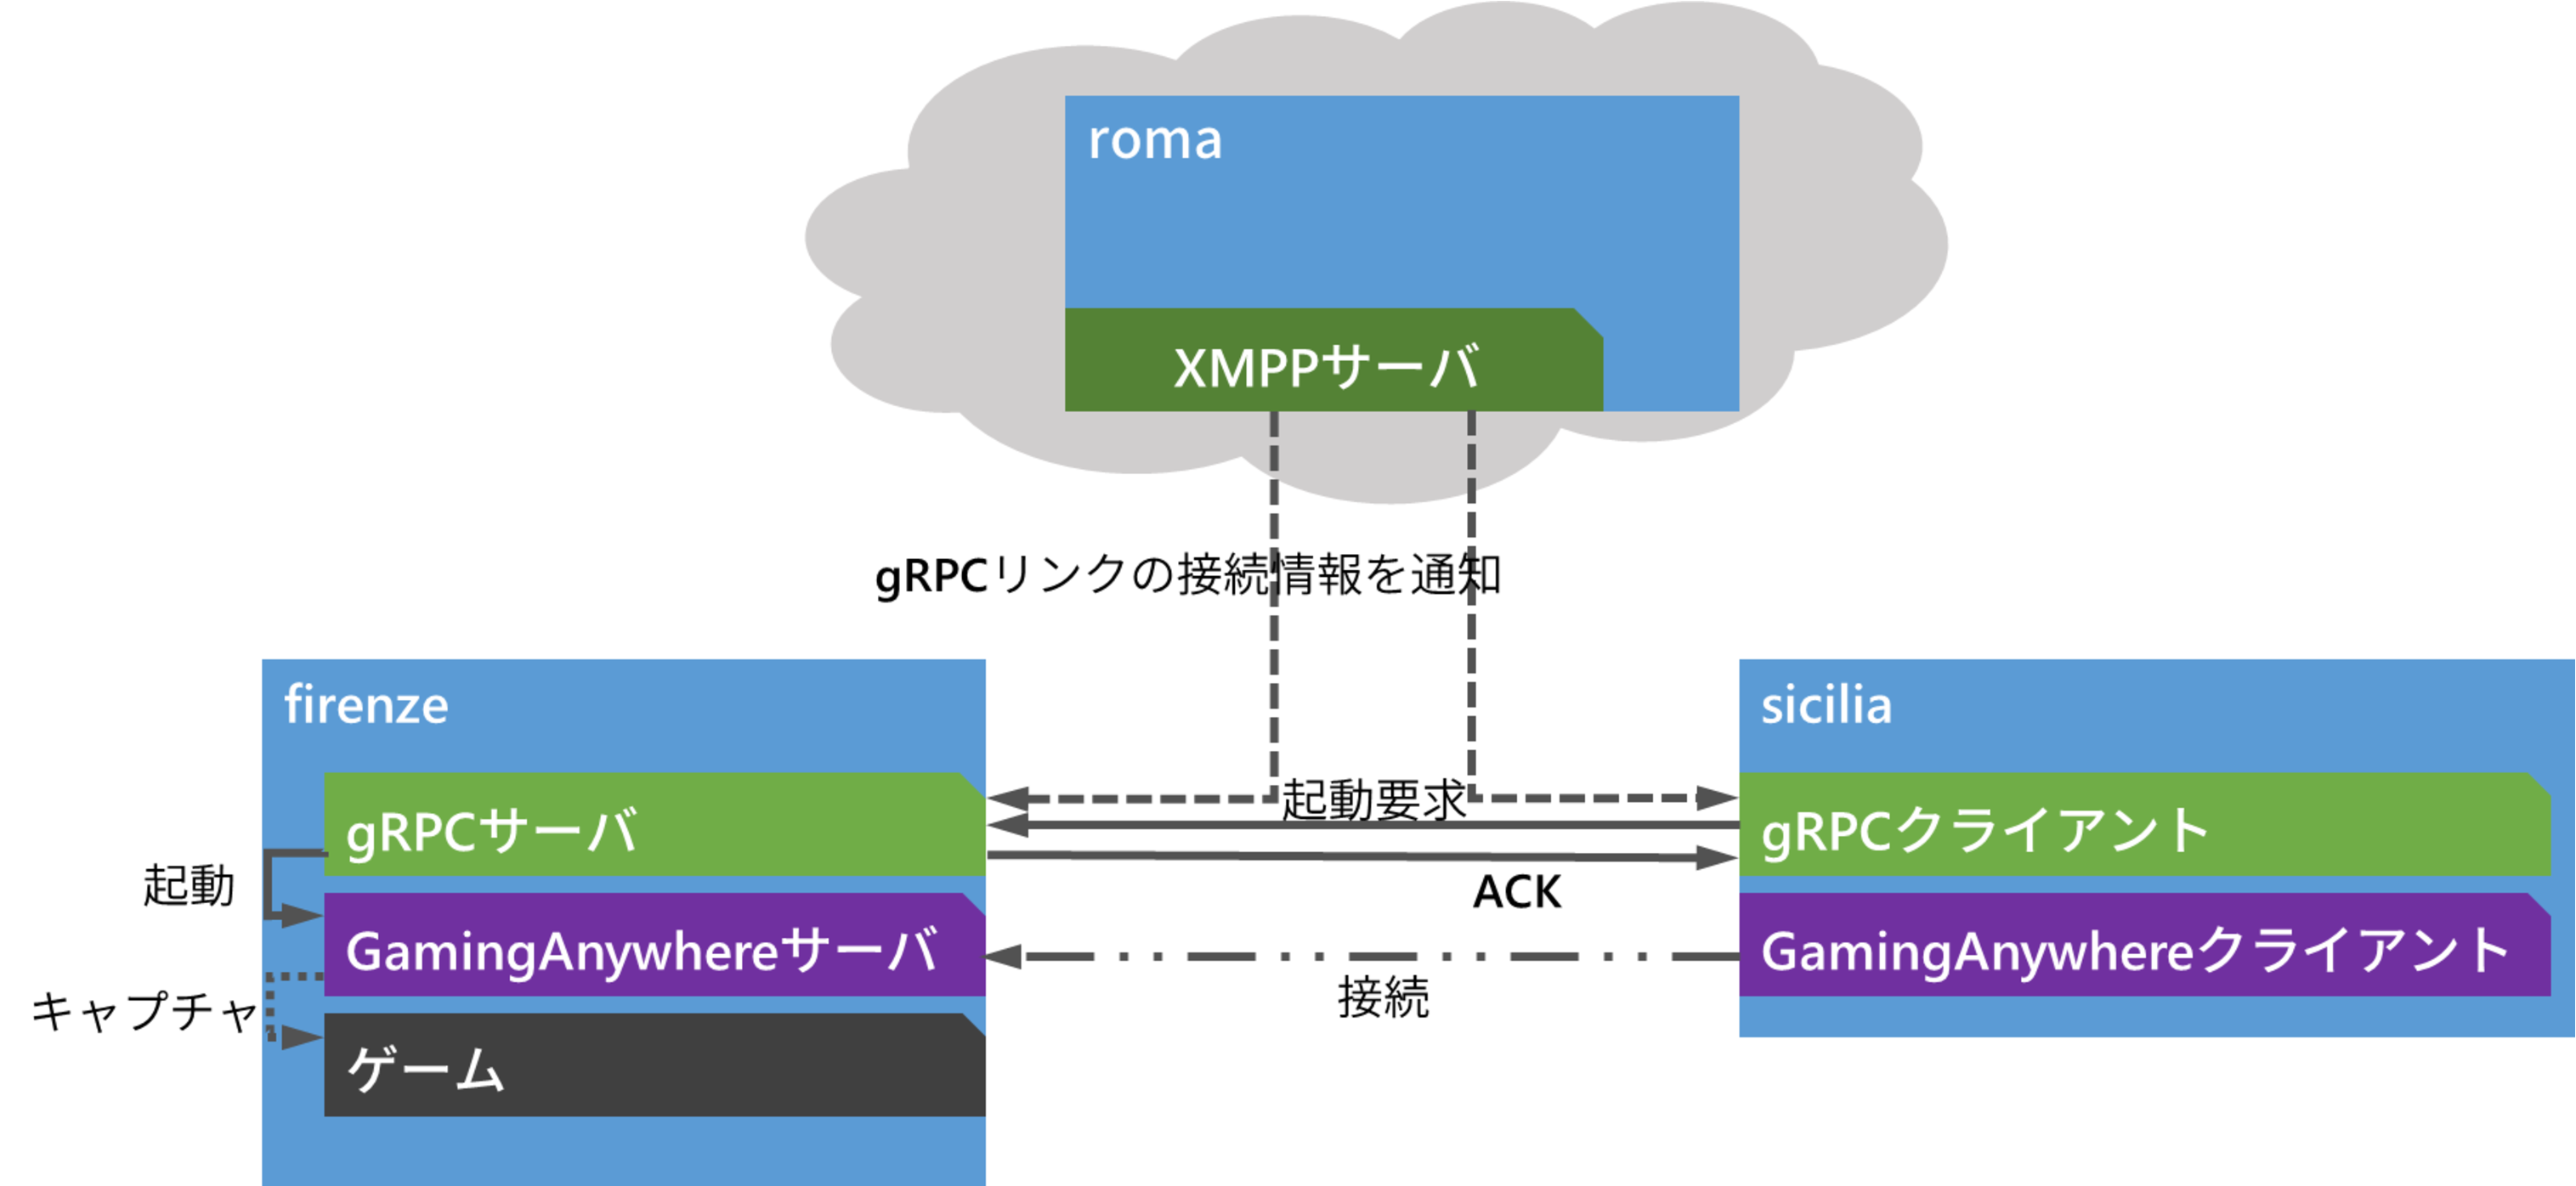
\includegraphics[width=0.8\textwidth,keepaspectratio,clip]{img/experimentalenvironment.eps}
    \caption{評価環境}
    \label{fig:expenv}
\end{figure*}

\subsection{クラウドゲームサーバ/クライアント間の通信性能}

\subsubsection{リンクに対する生の遅延の大小の影響}
siciliaとfirenzeの間のネットワーク遅延の大小によって、GamingAnywhereサーバ/クライアント間のリンクを張るために使用しているEdgeVPNのオーバーヘッドがリンクの遅延に与える影響について調査した。tc\cite{iproute2}を用いてリンクに0-60msの遅延を挿入し、EdgeVPNを利用する場合と直接接続する場合の遅延増加の様子ping\cite{ping}を用いて計測した。計測遅延と挿入遅延の値の差をプロットしたものが図\ref{fig:ratency}である。計測値にはpingを10回実行した際の値の平均値を使用している。

直接通信に比べて、EdgeVPNを利用する場合は平均して1ms程度遅延のオーバヘッドが存在することがわかる。また、遅延のオーバーヘッドは挿入遅延の大きさに関わらずほぼ一定であるといえる。

\begin{figure*}[t]
    \centering
    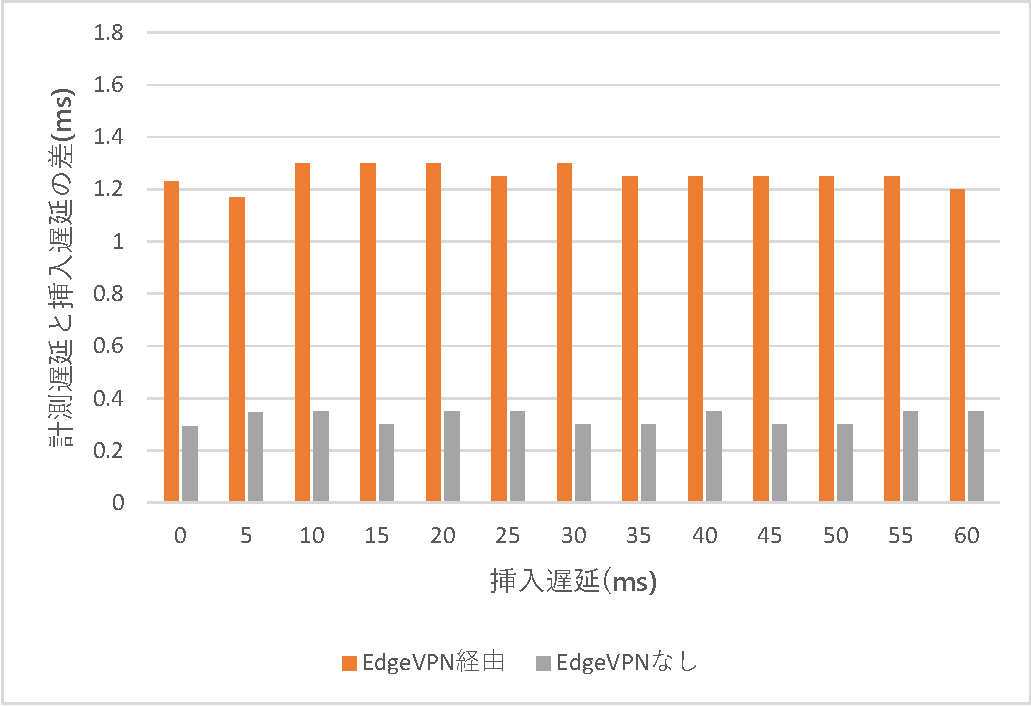
\includegraphics[width=0.8\textwidth,keepaspectratio,clip]{img/graph_ratency.pdf}
    \caption{EdgeVPNリンクに対する遅延挿入の影響}
    \label{fig:ratency}
\end{figure*}

\subsubsection{リンクに対する遅延の大小のスループットへの影響}
siciliaとfirenzeの間のネットワーク遅延の大小の影響で、GamingAnywhereサーバ/クライアント間のリンクで展開したEdgeVPNがリンクのネットワークスループットに与える影響について調査した。5.2.1と同様にtcを用いてリンクに0-60msの遅延を挿入し、EdgeVPNを利用する場合と直接接続する場合の帯域減少の様子をiperf\cite{iperf}を使用して計測した。計測値はiperfを60秒間の設定で10回実行した結果を用いている。EdgeVPNを利用する通信についての結果をプロットしたものが図\ref{fig:band_with_edge}、直接接続する通信についての結果をプロットしたものが図\ref{fig:band_without_edge}である。

EdgeVPNを利用する通信において、スループットが指数関数的に減少していることがわかる。一方で、最も大きい60msまで遅延が増大した状況下においても40Mbps程度のスループットをGamingAnywhereサーバ/クライアント間のリンクにおいて維持できている。(これは許容量であるみたいなことを関連研究のとこ書いてから書く)

\begin{figure*}[t]
    \centering
    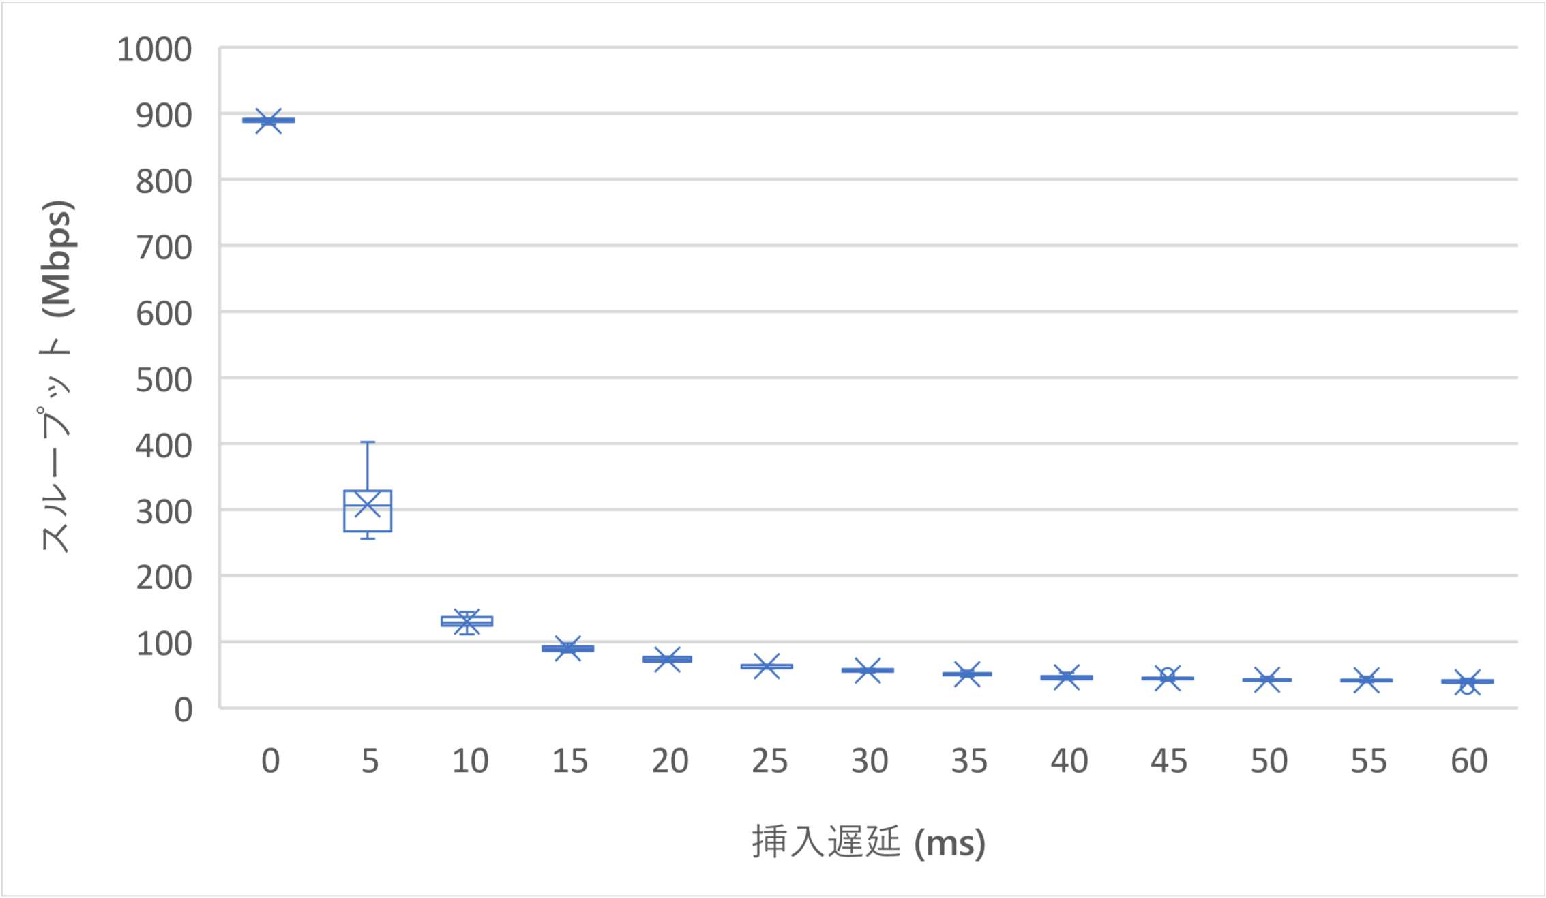
\includegraphics[width=0.8\textwidth,keepaspectratio,clip]{img/bandwidth_withEdgeVPN.pdf}
    \caption{EdgeVPNリンクへの遅延挿入の帯域への影響}
    \label{fig:band_with_edge}
\end{figure*}

\begin{figure*}[t]
    \centering
    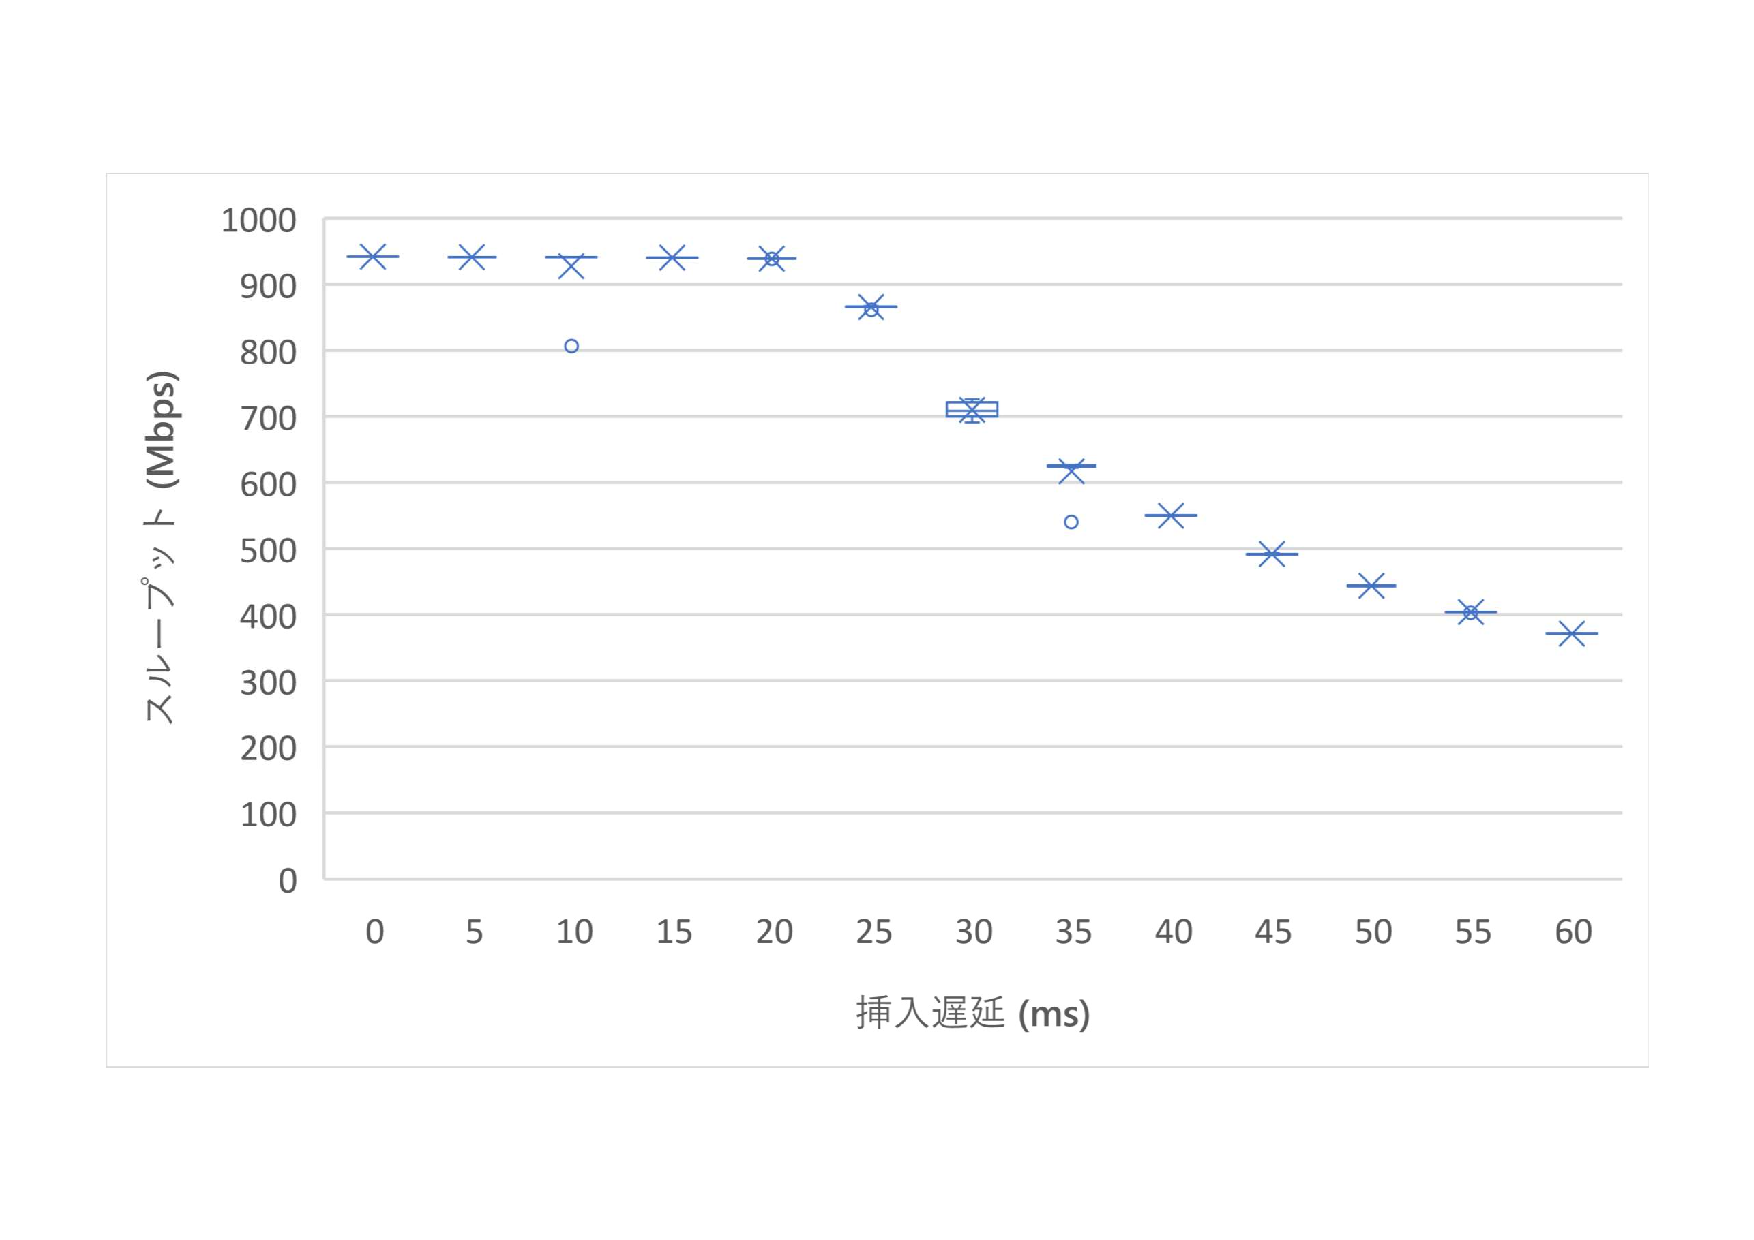
\includegraphics[width=0.8\textwidth,keepaspectratio,clip]{img/bandwidth_withoutEdgeVPN.pdf}
    \caption{EdgeVPNを使用していないリンクへの遅延挿入の帯域への影響}
    \label{fig:band_without_edge}
\end{figure*}

\subsection{ゲームプレイ時のフレームレート}

\subsubsection{ネットワーク帯域の大小の影響}
提案システムを使用して実際にゲームをプレイしている間、siciliaとfirenzeの間のネットワーク帯域幅のサイズがゲーム画面のフレームレートにどのように影響するかを調査した。

実験はGamingAnywhereサーバの設定でフレームレートを60fpsに設定した状態で行った。ゲームのジャンルにより画面の動きが激しく、フレームレートの変動の影響が大きいものとそうでないものがあるため、複数のジャンルから選んだゲームを実験に使用した。実験に使用したゲームはMMORPGに分類されるAlbion Online\cite{albiononline}、FPS/アクションに分類されるRed Eclipse 2\cite{redeclipse}、およびボードゲームであるSimply Chess\cite{simplychess}の3種類である。いずれもPCゲームのダウンロード販売等を行うプラットフォームであるSteam\cite{steam}で公開されている、Linuxに対応したゲームである。

GamingAnywhereサーバ/クライアント間のリンクにtcを使用して帯域制限を施し、EdgeVPNを利用する場合と直接接続する場合のそれぞれについてフレームレートの変化を観測した。帯域制限は、制限をかけていない1Gbpsおよび100Mbpsと10Mbpsの3つの条件で行った。計測値はGamingAnywhereクライアントが定期的に出力するフレームレートの値を10回分計測し、その平均値を使用している。Albion Onlineをプレイした際の結果を図\ref{fig:fps_mmo}、Red Eclipse 2をプレイした際の結果を図\ref{fig:fps_fps}、Simply Chessをプレイした際の結果を図\ref{fig:fps_board}にそれぞれ示した。

動きのあまり少ないボードゲームのSimply Chessのプレイ中においてはEdgeVPNを利用するかどうかに関わらず、帯域制限下でもほぼ60fpsのフレームレートを保っている。また、常に画面の少なくとも一部に動きが生じるジャンルであるMMORPGのAlbion Onlineのプレイ中においても、帯域制限下で60fpsを大きく下回ることなくパフォーマンスが安定している。さらに、常に画面全体に激しい動きが発生するFPS/アクションに分類されるRed Eclipse 2のプレイ中においても、帯域制限下でフレームレートの低下は確認されなかった。

\begin{figure*}[t]
    \centering
    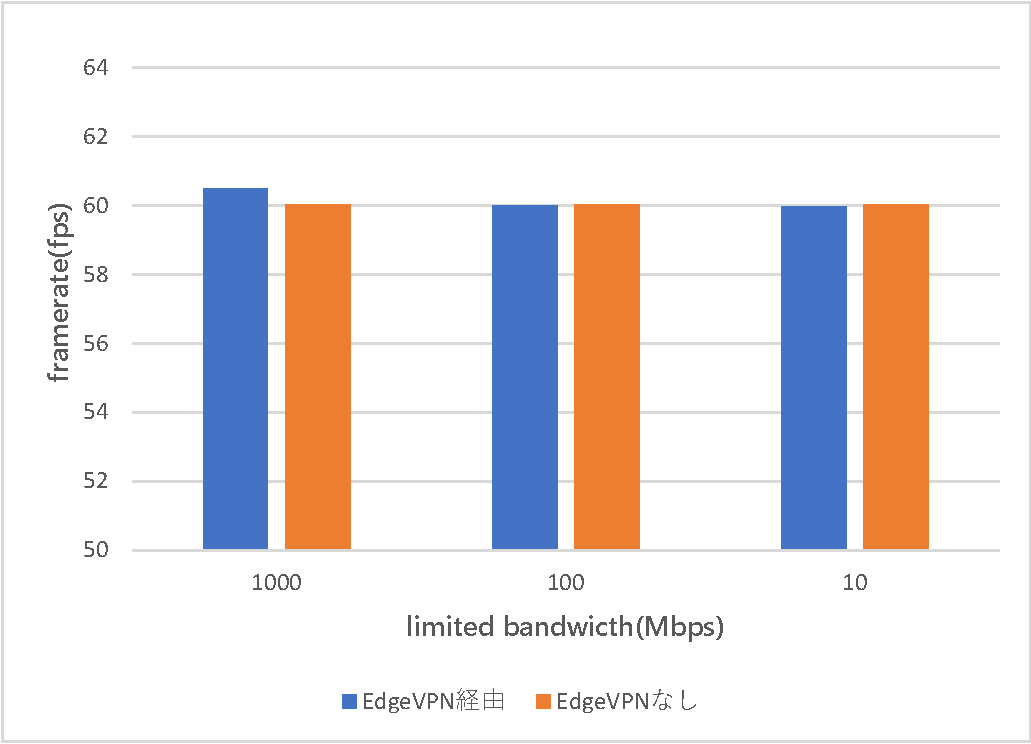
\includegraphics[width=0.8\textwidth,keepaspectratio,clip]{img/framerate_MMO.pdf}
    \caption{帯域制限下でのゲームプレイ時のフレームレートの変化 (Albion Online (MMORPG)プレイ時)}
    \label{fig:fps_mmo}
\end{figure*}

\begin{figure*}[t]
    \centering
    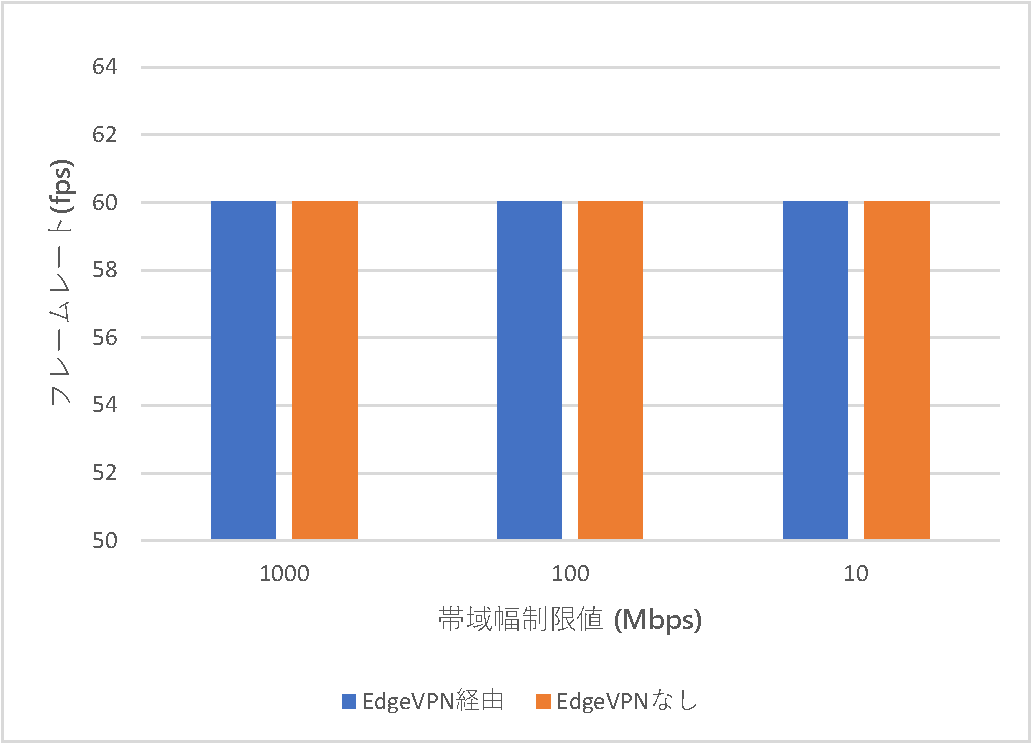
\includegraphics[width=0.8\textwidth,keepaspectratio,clip]{img/framerate_FPS.pdf}
    \caption{帯域制限下でのゲームプレイ時のフレームレートの変化 (Red Ecliplse 2 (FPS, Action)プレイ時)}
    \label{fig:fps_fps}
\end{figure*}

\begin{figure*}[t]
    \centering
    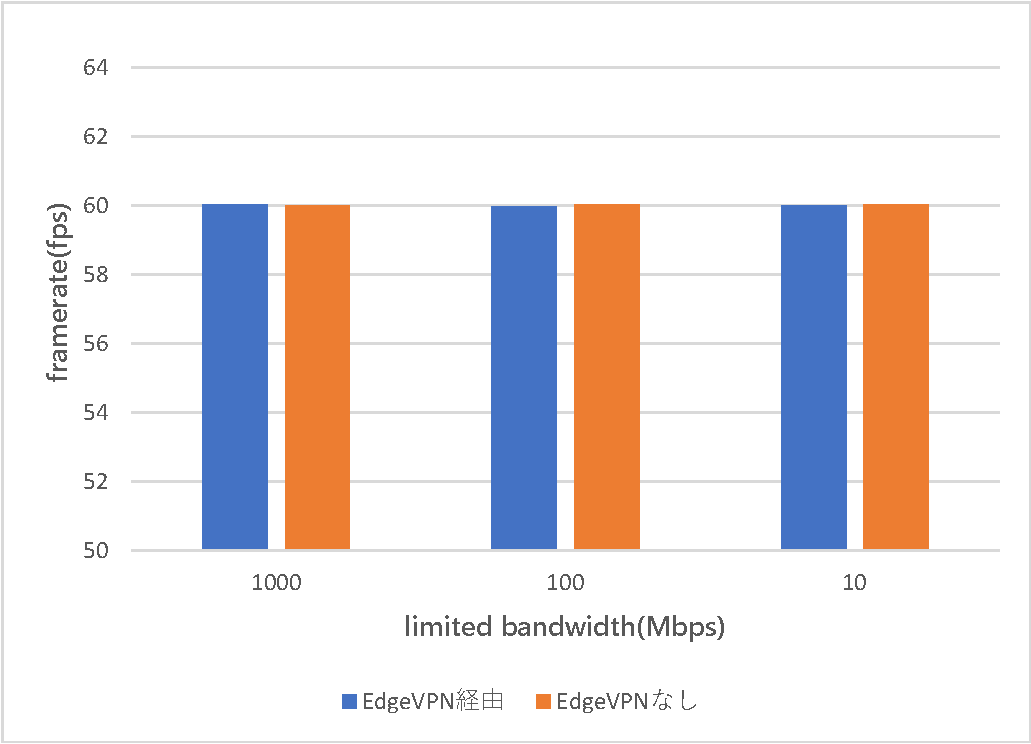
\includegraphics[width=0.8\textwidth,keepaspectratio,clip]{img/framerate_Board.pdf}
    \caption{帯域制限下でのゲームプレイ時のフレームレートの変化 (Simply Chess (ボードゲーム)プレイ時)}
    \label{fig:fps_board}
\end{figure*}

\subsection{考察}
どれぐらい数値が良ければ既存に勝てるのかみたいなこと



